\input{preamble.sty}

\title{Лабораторная работа №2. Ручное построение нисходящих синтаксических анализаторов}
\author{Михайлов Максим, группа M3337 \\ Вариант 9: описание заголовка функции в Kotlin}

\let\endtitlepage\relax

\begin{document}

\maketitle
\thispagestyle{empty}

\section{Построение грамматики}

Построим интуитивную грамматику.

\begin{minipage}{.2\textwidth}
    \begin{align*}
        H & \to \texttt{fun}\ N\texttt{(}P\texttt{)}R \\
        P & \to N\ T\texttt{,} P                      \\
        P & \to N\ T                                  \\
        P & \to \varepsilon                           \\
        T & \to {}\texttt{:} N                        \\
        R & \to T                                     \\
        R & \to \varepsilon
    \end{align*}
\end{minipage}
\begin{minipage}{.8\textwidth}
    \begin{center}
        \begin{tabular}{Ll}
            \toprule
            \text{Нетерминал} & Описание                  \\ \midrule
            H                 & Заголовок функции         \\
            % N                 & Идентификатор                               \\
            P                 & Список параметров функции \\
            T                 & Аннотация типа            \\
            R                 & Возвращаемый тип          \\
            \bottomrule
        \end{tabular}
    \end{center}
\end{minipage}

В этой грамматике есть правое ветвление для \(P\). Устраним правое ветвление:

\begin{minipage}{.2\textwidth}
    \begin{align*}
        H  & \to \texttt{fun}\ N\texttt{(}P\texttt{)}R \\
        P  & \to N\ T\ P'                              \\
        P  & \to \varepsilon                           \\
        P' & \to \varepsilon                           \\
        P' & \to \texttt{,} P                          \\
        T  & \to {}\texttt{:} N                        \\
        R  & \to T                                     \\
        R  & \to \varepsilon
    \end{align*}
\end{minipage}
\begin{minipage}{.8\textwidth}
    \begin{center}
        \begin{tabular}{Ll}
            \toprule
            \text{Нетерминал} & Описание                        \\ \midrule
            H                 & Заголовок функции               \\
            P                 & Список параметров функции       \\
            P'                & Хвост списка параметров функции \\
            T                 & Аннотация типа                  \\
            R                 & Возвращаемый тип                \\
            \bottomrule
        \end{tabular}
    \end{center}
\end{minipage}

\section{Построение лексического анализатора}

\definecolor{bg}{rgb}{0.95,0.95,0.95}
Создадим класс \texttt{Token} для хранения терминалов.
\inputminted[bgcolor=bg]{kotlin}{lab2/src/main/kotlin/Token.kt}
\begin{center}
    \begin{tabular}{ll}\toprule
        Терминал     & Токен               \\ \midrule
        \texttt{fun} & \texttt{FUN}        \\
        \(N\)        & \texttt{IDENTIFIER} \\
        \texttt{(}   & \texttt{LPAREN}     \\
        \texttt{)}   & \texttt{RPAREN}     \\
        \texttt{,}   & \texttt{COMMA}      \\
        \(\$\)       & \texttt{END}        \\
        \bottomrule
    \end{tabular}
\end{center}

\inputminted[bgcolor=bg]{kotlin}{lab2/src/main/kotlin/LexicalAnalyzer.kt}

\section{Построение синтаксического анализатора}

Построим множества FIRST и FOLLOW для нетерминалов нашей грамматики.

\begin{center}
    \begin{tabular}{LLL} \toprule
        \text{Нетерминал} & \text{FIRST}            & \text{FOLLOW}              \\ \midrule
        H                 & \texttt{fun}            & \$                         \\
        % N                 &           &                   \\
        P                 & \varepsilon, N          & \texttt{)}                 \\
        P'                & \varepsilon, \texttt{,} & \texttt{)}                 \\
        T                 & \texttt{:}              & \texttt{)}, \texttt{,}, \$ \\
        R                 & \varepsilon, \texttt{:} & \$                         \\
        \bottomrule
    \end{tabular}
\end{center}

Заведем структуру данных для хранения дерева и парсер.

\inputminted[bgcolor=bg]{kotlin}{lab2/src/main/kotlin/Parser.kt}

\section{Визуализация дерева разбора}

\begin{figure}[h]
    \centering
    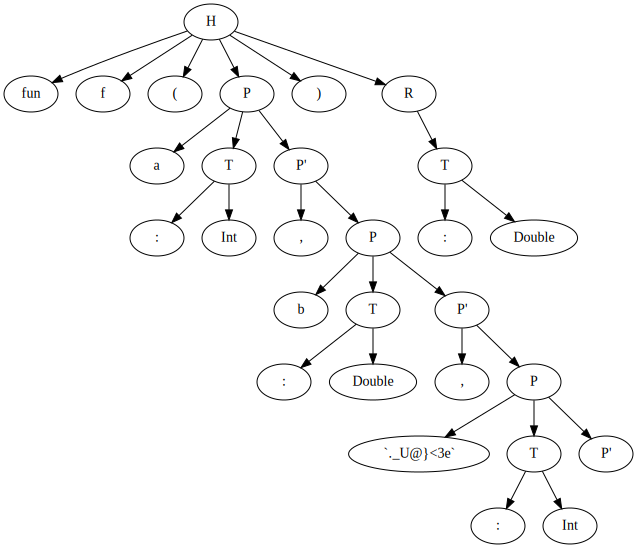
\includegraphics[scale=0.4]{lab2/tree.png}
    \caption{Пример дерева разбора для\\\texttt{fun f(a: Int, b: Double, `\~{}o4ahi=M`: Int):Double}}
\end{figure}

\inputminted[bgcolor=bg]{kotlin}{lab2/src/main/kotlin/Main.kt}

\section{Подготовка набора тестов}

\begin{center}
    \begin{tabular}{ll}\toprule
        Тест                                    & Описание                                     \\ \midrule
                                                & Пустой тест (должен произвести ошибку)       \\
        \texttt{fun f(a: Int, b: Bool): Double} & Небольшой случайный пример                   \\
        \texttt{fun f(a: Int, b: Bool)}         & Тест без возвращаемого типа                  \\
        \texttt{fun f(): Double}                & Тест без параметров                          \\
        \texttt{fun f()}                        & Тест без параметров и возвращаемого типа     \\
        \texttt{fuuun f()}                      & Тест с неверным ключевым словом \texttt{fun} \\
        \texttt{fun \_F1\_a2(`'g[4]VA?`: Int)}  & Тест с экранированным идентификатором        \\
        \texttt{fun f(a: Int):}                 & Тест с двоеточием для типа, но без типа      \\
        \texttt{fun f(a: Int): 1}               & Тест с неверным идентификатором              \\
        \texttt{fun f(a: 1)}                    & Тест с неверным идентификатором              \\
        \texttt{fun f(1: Int)}                  & Тест с неверным идентификатором              \\
        \texttt{fun 1()}                        & Тест с неверным идентификатором              \\
        \texttt{fun f(a: Int,)}                 & Тест с висящей запятой                       \\
        \texttt{fun f(, a: Int)}                & Тест с неверно расположенной запятой         \\
        \bottomrule
    \end{tabular}
\end{center}

\end{document}
